\documentclass[11pt,a4paper]{article}
\usepackage[margin=1in]{geometry}
\usepackage{graphicx}
\usepackage{float}
\usepackage{amsmath}
\usepackage{hyperref}

\title{EN3160 Computer Vision Assignment 02\\Fitting and Alignment Report}
\author{Savindu Wickramasinghe \\ Index No.: 220701X}
\date{\today}

\begin{document}

\maketitle

\section{Introduction}
This report summarizes the implementation and results of four core fitting and alignment tasks completed for EN3160 Computer Vision Assignment 02. The experiments cover sunflower blob detection with the Laplacian of Gaussian (LoG), RANSAC-based primitive fitting, single homography-based image warping, and wide-baseline image stitching. All code was developed in Python with OpenCV, scikit-image, NumPy, and Matplotlib.

\section{Sunflower Blob Detection}
The objective was to localize prominent sunflowers in the aerial photograph \texttt{the\_berry\_farms\_sunflower\_field.jpeg}. The workflow converted the image to grayscale and applied the LoG detector \cite{lindeberg1994scale}. Key parameters were \(\texttt{min\_sigma} = 10\), \(\texttt{max\_sigma} = 40\), \(\texttt{num\_sigma} = 10\), and a detection threshold of 0.1. Detected blobs were ranked by radius and the five largest detections were reported to highlight the most prominent flowers. The resulting overlay demonstrates clean localization with minimal false positives around the field center where sunflowers dominate the scene.

\begin{figure}[H]
  \centering
  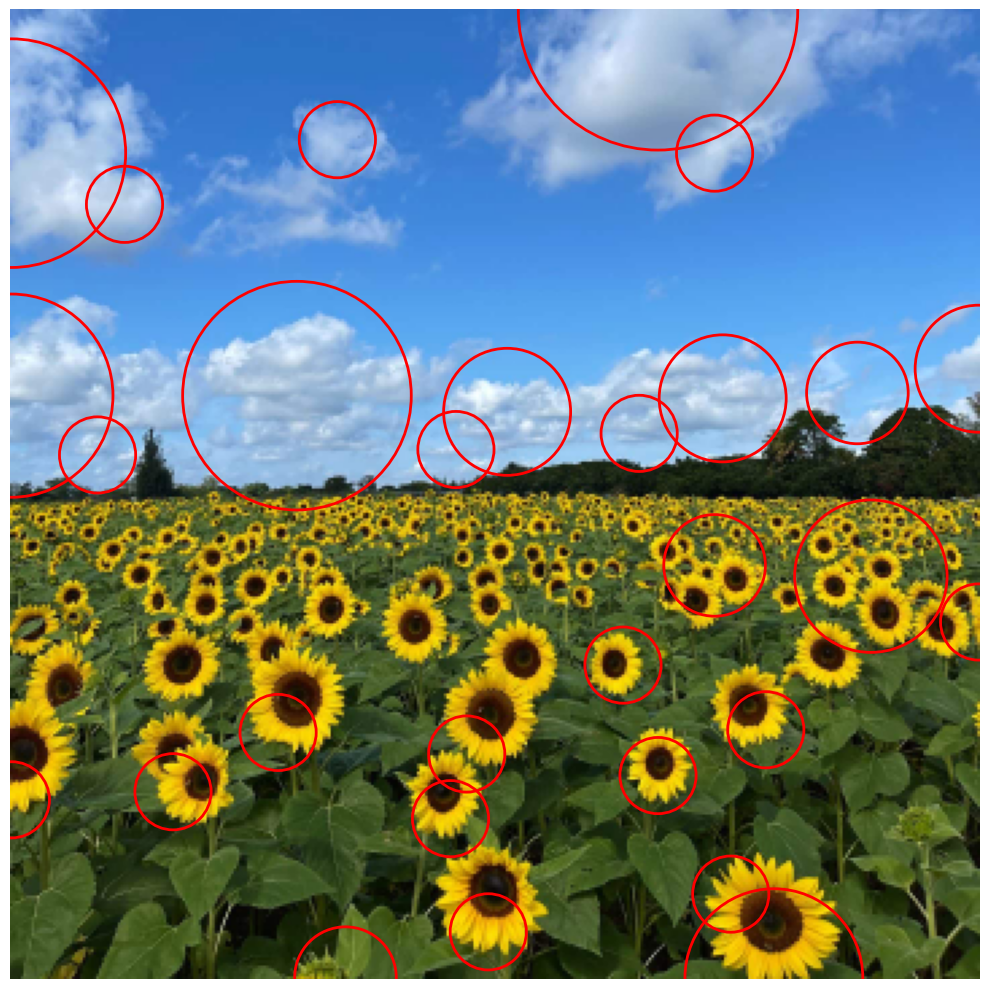
\includegraphics[width=0.85\linewidth]{sunflower_detection.png}
  \caption{Sunflower detections obtained with the LoG detector. Red circles indicate detected flower heads.}
  \label{fig:sunflower}
\end{figure}

\section{RANSAC-Based Primitive Fitting}
A synthetic dataset combining inliers from a noisy circle and a noisy line, along with additional outliers, was generated to evaluate robust fitting. Two custom RANSAC pipelines were executed sequentially: a line model estimated from minimal two-point samples followed by singular value decomposition (SVD) refinement, and a circle model estimated from three-point samples solved via linear algebra. Adaptive inlier thresholds of 0.5 for the line and 0.8 for the circle were sufficient to recover accurate models despite significant contamination. Figure~\ref{fig:ransac} shows the recovered primitives and their inlier sets.

\begin{figure}[H]
  \centering
  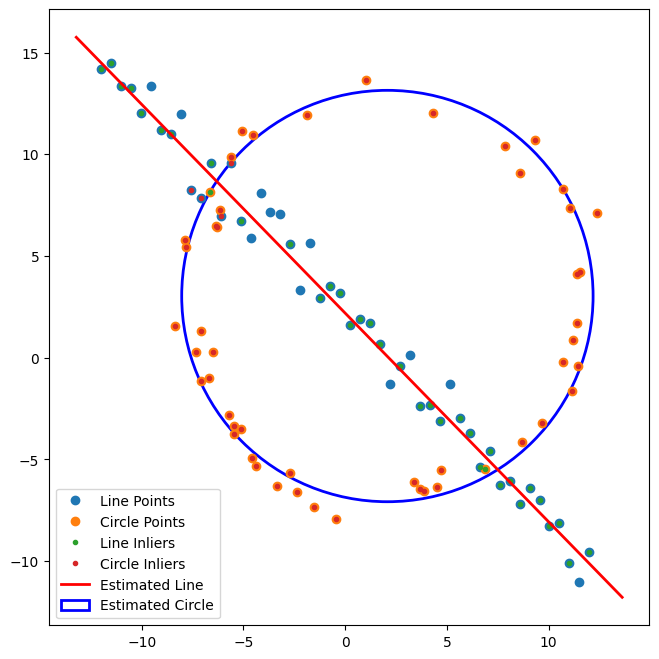
\includegraphics[width=0.7\linewidth]{ransac_fit.png}
  \caption{RANSAC fitted line and circle. Green and blue markers denote inlier assignments, while the magenta line and red circle are the refined models.}
  \label{fig:ransac}
\end{figure}

\section{Homography-Based Logo Warping}
To practice planar image alignment, a synthetic building facade \texttt{my\_building.png} and a solid-color logo \texttt{my\_logo.png} were used. Four corresponding corner points were manually selected on the destination image, defining a homography that maps the logo's corners to those locations. The homography was applied with \texttt{cv2.warpPerspective}, and the warped logo was alpha-composited onto the building using a polygon mask. The process demonstrates how planar inserts can be convincingly overlaid on a target surface.

\begin{figure}[H]
  \centering
  
\includegraphics[width=0.45\linewidth]{my_building.png}
  \hfill
  
\includegraphics[width=0.45\linewidth]{my_logo.png}
  \caption{Source imagery for the homography experiment. Left: destination building facade. Right: source logo to be warped.}
  \label{fig:homography_inputs}
\end{figure}

\begin{figure}[H]
  \centering
  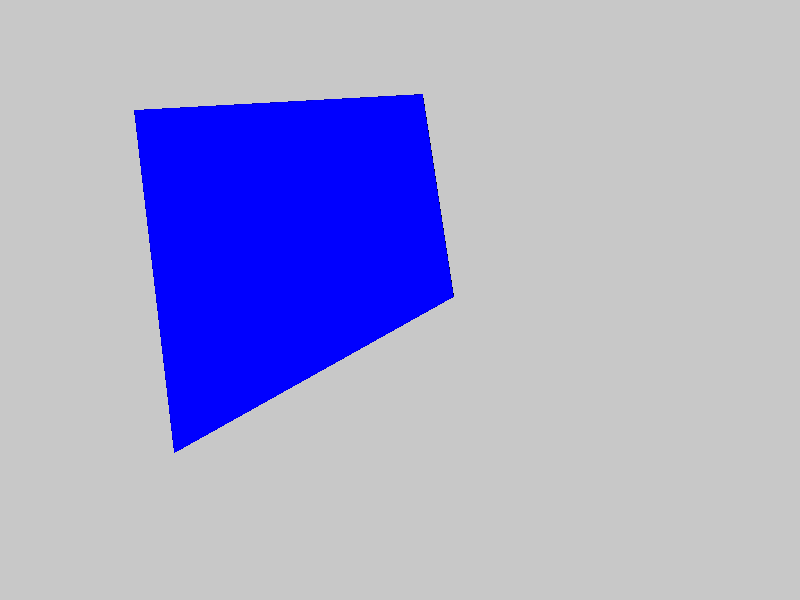
\includegraphics[width=0.7\linewidth]{homography_result.png}
  \caption{Result after warping the logo onto the building facade using the estimated homography.}
  \label{fig:homography_result}
\end{figure}

\section{Image Stitching}
The final task stitched the wide-baseline \texttt{graf/img1.ppm} and \texttt{graf/img5.ppm} views. Scale-Invariant Feature Transform (SIFT) descriptors were extracted on both images and paired with a FLANN-based matcher using Lowe's ratio test (0.7). The surviving correspondences fed into OpenCV's RANSAC homography estimator with a reprojection threshold of 5 pixels. The left image was warped into the right image's reference frame and composited to produce a wide field-of-view mosaic, shown in Figure~\ref{fig:stitching}.

\begin{figure}[H]
  \centering
  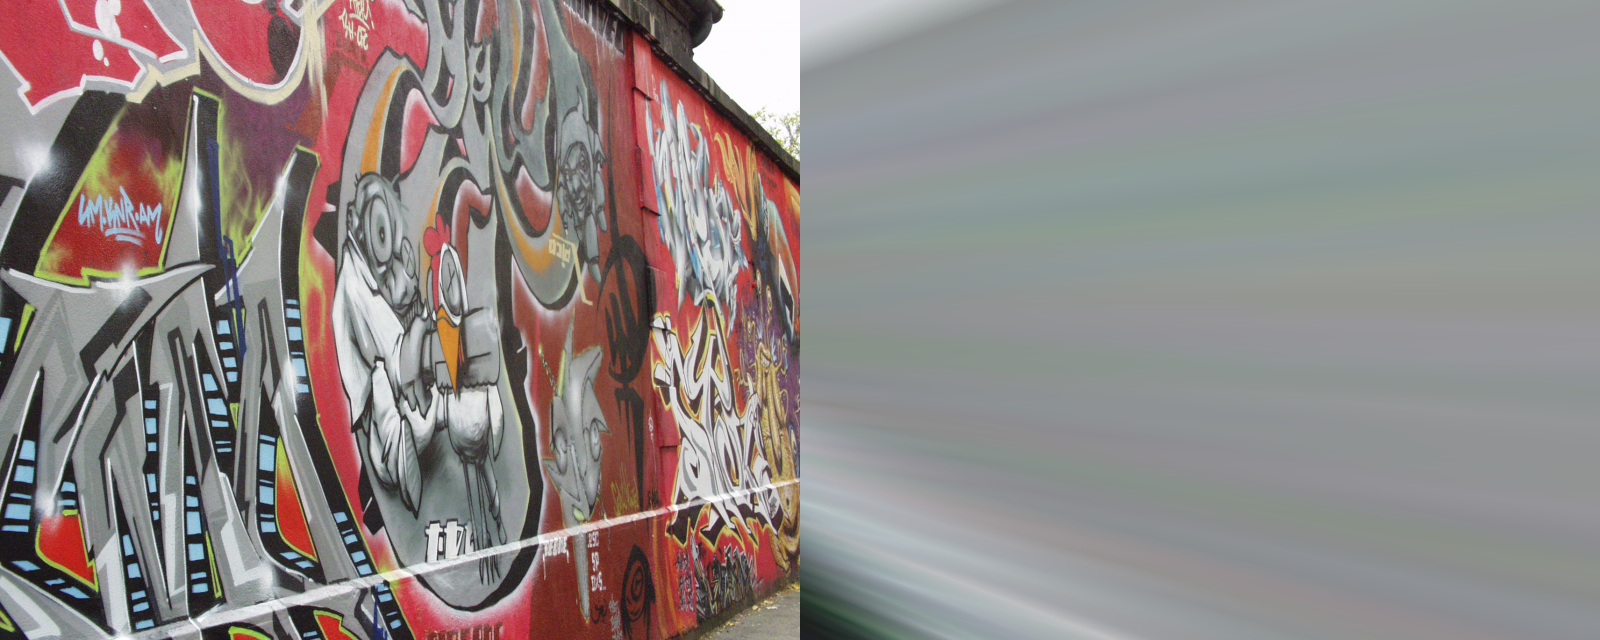
\includegraphics[width=0.9\linewidth]{stitching_result.png}
  \caption{Two-view panorama generated from the \texttt{graf} dataset. The seam falls outside the overlapping textured regions, yielding a visually coherent stitch.}
  \label{fig:stitching}
\end{figure}

\section{Conclusion}
Across the four experiments, classical computer vision techniques delivered reliable alignment results. Multi-scale LoG detection successfully isolated sunflowers, bespoke RANSAC pipelines robustly separated line and circle structures, planar homographies enabled controlled logo insertion, and feature-based stitching produced a wide-baseline panorama. Future work could explore automatic corner selection for homography synthesis and multiband blending to further reduce visible seams in stitched mosaics.

\bibliographystyle{plain}
\begin{thebibliography}{1}

\bibitem{lindeberg1994scale}
Tony Lindeberg.
\newblock Scale-space theory: A basic tool for analyzing structures at different scales.
\newblock \emph{Journal of Applied Statistics}, 21(1--2):225--270, 1994.

\end{thebibliography}

\end{document}
